\section{Implementation}\label{sec:implement}

%-----------------------------------------------------------------------------
\subsection{Omni XMP Compiler Framework}
%-----------------------------------------------------------------------------

The CAF translator was added to the Omni XMP compiler~\cite{omni}, 
as shown in Figure~\ref{fig:translator}.
The Omni XMP compiler is a source-to-source translator that converts XMP programs 
into the base language (Fortran or C). The component 'coarray translator' is 
located in front of the XMP translator to solve coarray features previously.   
The output of the decompiler is a standard Fortran/C program, which may include 
calls to the XMP runtime library.

The following procedures are generated in advance or in the coarray translator
to initialize static coarray variables prior to the execution of the user program:
\begin{itemize}
\item
The built-in main program calls subroutine {\tt xmpf\_traverse\_init},
the entry procedure of initialization subroutines, before executing the
user main program.
\item
Subroutine {\tt xmpf\_traverse\_init} is generated by the coarray translator 
to call initialization subroutines corresponding to all user-defined procedures.
\item
Each initialization subroutine {\tt xmpf\_init\_{\it foo}} is generated from 
user-defined procedure {\it foo} by the coarray translator, which initializes all static coarrays declared in {\it foo}.
\end{itemize}

\begin{figure}[tbh]
 \begin{center}
  % trimはleft bottom right topの順
  %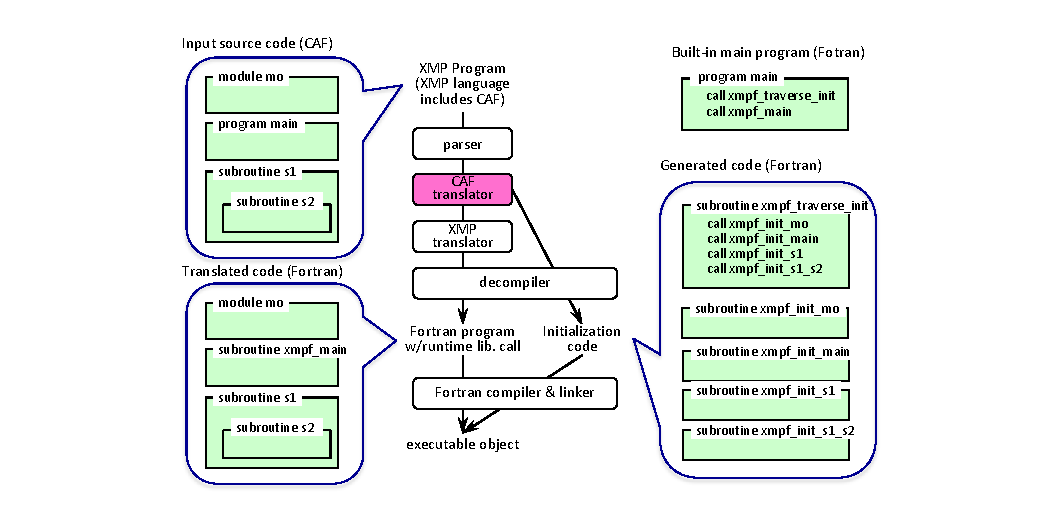
\includegraphics[scale=0.55,trim=6cm 0cm 4cm 6cm,clip]{figs/translator-tmp.pdf}
  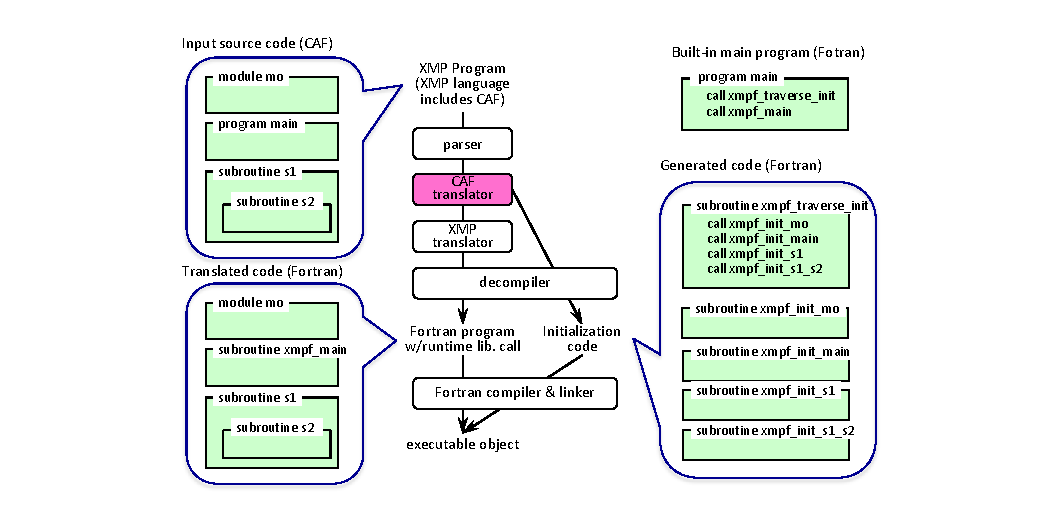
\includegraphics[trim=30mm 0mm 20mm 7mm, scale=1.0]{figs/translator-tmp.pdf}
  \caption{XMP compiler and an example of coarray program compilation}
  \label{fig:translator}
  %-- 修正すべき箇所
  CAF translator $\rightarrow$ coarray translator
 \end{center}
\end{figure}


%-----------------------------------------------------------------------------
\subsection{Allocation and Registration}\label{sec:alloc}
%-----------------------------------------------------------------------------

In order to be accessed using the underlying communication library,
the allocated coarray data must be registered to the library.
The registration contains all actions to allow the data to be accessed 
from the other nodes, including pin-down memory, acquirement of the global address,
and sharing information among all nodes.

%===========================================================
\subsubsection{Three Methods of Memory Management}
%===========================================================

The coarray translator and the runtime library implements three methods of
memory management.
\begin{itemize}
\item
The {\bf runtime sharing (RS) method} allocates and registers a large memory 
for all static and dynamic coarrays at the initialization phase.
The registered memory is shared by all static and allocatable coarrays. 

\item
The {\bf runtime allocation (RA) method} allocates and registers a large memory
for all static coarrays at the initialization phase.
The RA method also allocates and registers each allocatable coarray at runtime.

\item
The {\bf compiler allocation (CA) method} allocates all coarray objects by 
the Fortran system (at compile time or at runtime), and the address is 
passed to the runtime library to be registered.
\end{itemize}

For the RS and RA methods, 
since the allocated memory address is determined in the runtime library, 
the object code must accept the address allocated 
inside the runtime system as an address of a regal Fortran variable.
To make this connection, it was necessary to use the Cray pointer, which is not 
in the Fortran standard.
In the case of the CA method, the runtime library accepts the address allocated
in the Fortran system and registers to the communication library.

%
% 3 methodsの比較表を載せるならここか
%


%===========================================================
\subsubsection{Initial Allocation for Static Coarrays}
%===========================================================

Static coarrays are allocated and registered in the initialization subroutines 
{\tt xmpf\_init\_{\it foo}}. 

Using the RS and RA methods, static coarrays are initialized before execution of the user program,
as follows.
\begin{itemize}
\item
In the first pass, all sizes of static (non-allocatable) coarrays are summed.
The size of each static coarray is evaluated form the lower and upper bounds
specified in the dimension declaration statement of each coarray.
The lower and upper bound expressions, possibly including binary and unary
operations, references to names of constants, and basic intrinsic functions, 
such as min/max and sum, are evaluated by constant folding.
Since the size of the structure that contains allocatable or pointer 
components differs depending on the target compiler, the coarray translator
obtains the necessary parameters to calculate the size of structures at build time.
\item
Then, the total size of static coarrays is allocated and the address
and size are registered to the underlying communication library.
\item
In the second pass, the addresses of all of the coarrays are calculated to share
the registered data.
Due to the language specification, the sizes of the same coarray are the same 
among all images (nodes). Therefore, the offset from the base address of the registered 
data for each coarray can be the same among all images.
\end{itemize}
%
In the RS method, allocatable coarrays also share the registered memory. 
The total size of the memory to be registered
should be specified with an environment variable by the user.
In the RA method, the total size is fully calculated by the runtime 
library, and no information is required of the user because allocatable coarrays
will be dynamically allocated on the other memories.

In the CA method,
the Fortran processor allocates each coarray, and the runtime library
then registers the address.
Each static coarray is converted into a common (external) variable to share 
between the user-defined procedure (say {\it foo}) and its initialization
procedure ({\tt xmpf\_init\_{\it foo}}). The data is statically allocated
by the Fortran system in a manner similar to the usual common variable.
The address is registered in the initialization procedure via the runtime library.

%===========================================================
\subsubsection{Runtime Allocation for Allocatable Coarrays}
%===========================================================

For the RS method, the runtime library has a memory management system for
cutting out and retrieving memory for each allocation and deallocation of coarrays.

Figure~\ref{fig:register-RA-CA} illustrates the memory allocation and registration
for allocatable coarrays in the RA and CA methods. 

\begin{figure}
 \begin{center}
  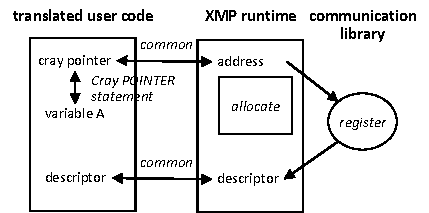
\includegraphics[scale=0.9, trim=0mm 0mm 0mm 0mm, clip]{figs/register-RA-tmp.pdf}\\
The runtime allocates and registers coarrays and passes the address to the user code.
 \end{center}
 \begin{center}
(a) RA method
 \end{center}
 \begin{center}
  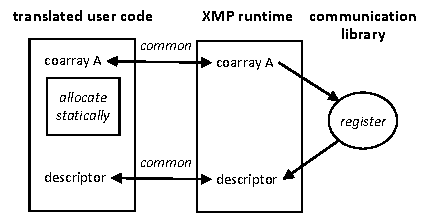
\includegraphics[scale=0.9, trim=0mm 0mm 0mm 0mm, clip]{figs/register-CA-tmp.pdf}\\
The user code allocates coarrays and causes the runtime to register with the address.
 \end{center}
 \begin{center}
(b) CA method
 \end{center}
 \caption{Memory allocation for coarrays in RA and CA methods}
 \label{fig:register-RA-CA}
\end{figure}

These methods are properly used by the underlying communication library.
%
For GASNet, only the RS method is adopted because its allocation function
can be used only once in the program.
%
For MPI-3, the CA method is not suitable because frequent 
allocation and deallocation of coarrays cause expensive creation and freeing of 
MPI windows.
%
In the case of FJ-RDMA, the RS method has no advantage over the other methods.
Since the allocated address is used for registration to FJ-RDMA, 
no advantage was found for managing memory outside of the Fortran system. 
The unusual connection through the Cray pointer causes degradation of 
the Fortran compiler optimization.


%-----------------------------------------------------------------------------
\subsection{PUT/GET Communication}\label{sec:putget}
%-----------------------------------------------------------------------------

In order to avoid disturbing the execution on the remote image, PUT and GET communications
are always implemented using remote direct memory access (RDMA) provided by 
the communication library (except coarrays with pointer/allocatable structure components). 
In contrast, local data access is selective between using direct memory access (DMA) or
using a local buffer. For the buffer scheme, one of four algorithms will be chosen.


%===========================================================
\subsubsection{Determining the Possibility of DMA}\label{sec:opt-dma}
%===========================================================

Coarray variables must be registered when allocated to be 
the target of RDMA communication. In contrast, since the local
data, which is the source of PUT or the destination of GET,
was not registered or linked to registered information,
the data could not be the target of DMA communication and had to be communicated via the registered buffer.

When the local data is an entire coarray or a part of coarray,
the coarray must be registered, and efficient DMA-RDMA communication can 
be made. Since the analysis at compile time is limited,
we implemented the detector in the runtime library 
using binary-tree search, as follows.
%
\begin{enumerate}
\item
When a chunk of coarray data is registered to the communication library, 
the runtime library adds the set of the local address and the size to a sorted 
table called {\tt SortedChunkTable}. The sort key is the local base address
of the data.
\item
When a chunk of coarray data is deregistered from the communication library, the 
runtime library deletes the record in {\tt SortedChunkTable}.
\item
When a PUT or GET runtime library is called corresponding to a reference/definition
to a coindexed object/variable, the local address is searched in {\tt SortedChunkTable}
with binary search. The local data is already registered if 
$addr_i \leq addr < addr_i + size_i$ for any $i$,
where $addr$ is the said local address and $add_i$ and $size_i$ are the
$i$-th address and size, respectively, in {\tt SortedChunkTable}.
\end{enumerate}

If the communication data is large, then the cost of procedure 3 is relatively small
and is worth using. 
If the data is small, then the buffering algorithm, as shown in \Sec{buffer}, may be better.


%===========================================================
\subsubsection{Buffering Communication Methods}\label{sec:buffer}
%===========================================================

For the buffer scheme, one of four algorithms will be chosen 
depending on three parameters: the size of the local buffer $B$ and the 
local and remote contiguous lengths $N_L$ and $N_R$, respectively.
Here, $B$ should be large enough to ignore communication latency overhead and we use
approximately 400 kilo-bytes by default. Unlike the case of MPI message passing,
coarray PUT/GET communication requires only one local buffer for any number of
other images.
Both $N_L$ and $N_R$ can be evaluated at runtime. The Fortran syntax guarantees 
that $N_L$ is a multiple of $N_R$ or $N_R$ is a multiple of $N_L$.
An algorithm to obtain the contiguous length is shown in a previous paper~\cite{pgas15}.

\tab{putget} summarizes our algorithm for PUT/GET communication for five cases.
The unit size is the chunk length of the PUT/GET communication.
Case~0 shows the algorithm using RDMA-DMA PUT/GET communication, and Cases~1 through~4 show the algorithms using RDMA and local-buffering. 
Due to its strict condition, the DMA scheme is rarely used.
In addition, this scheme is not always faster than the buffering scheme for Cases~2 and~3 because of the difference in the unit sizes. The advantage of Cases~2 and~3 is that the unit size 
is extended to a multiple of $N_L$ by gathering a number of short contiguous data in the buffer,
or by scattering from the buffer into a number of short contiguous data.

\begin{table}[tbh]
 \caption{Summary of the PUT/GET algorithm related to $N_L$, $N_R$, and $B$}
 \label{tab:putget}
 \begin{flushleft}
  \begin{tabular}{|@{~}c@{~}|c||@{~}c@{~}|@{~}c@{~}|}
\hline
Scheme &
Case &
Condition &
Unit size \\
\hline
\hline
DMA &
&
local data is registered &
$\min(N_L, N_R)$ \\
\hline
Buffering &
1 & 
$N_R \leq B,~ N_R \leq N_L$ &
$N_R$ \\
\cline{2-4}
&
2 &
$N_L < N_R \leq B$ &
$N_R$ \\
\cline{2-4}
&
3 &
$N_L < B < N_R$ &
multiple of $N_L$ ($\leq B$) \\
\cline{2-4}
&
4 &
$B < N_R,~ B \leq N_L$ &
$B$ (or less than $B$ at last) \\
\hline
  \end{tabular}
 \end{flushleft}
 \begin{flushleft}
  \begin{tabular}{|@{~}c@{~}|c||@{~~}l@{~~}|@{~~}l@{~~}|}
\hline
Scheme &
Case &
PUT action for each unit &
GET action for each unit \\
\hline
\hline
DMA &
&
put once &
get once \\
\hline
Buffering &
1 &
buffer once, and put once &
get once, and unbuffer once \\
\cline{2-4}
&
2 &
buffer for each $N_L$, and put once &
get once, and unbuffer for each $N_L$ \\
\cline{2-4}
&
3 &
buffer for each $N_L$, and put once &
get once, and unbuffer for each $N_L$ \\
\cline{2-4}
&
4 &
buffer once, and put once &
get once, and unbuffer once \\
\hline
  \end{tabular}
 \end{flushleft}
\end{table}


%===========================================================
\subsubsection{Non-blocking PUT Communication}
%===========================================================

For higher performance, the PUT communication should be non-blocking, and
the completion wait should be delayed until the end of the segment.
Writing and reading the same remote data from
the same image in the same segment appears to be a very rare case, as described in \Sec{spec-sync}.
However, this is difficult to detect with low cost. Since the subscripts and image
indices are often variable expressions, the compiler rarely select non-blocking communication
and usually generates safe but slow code.
We do not have a reasonable solution for this issue.

In the current implementation, the user selects blocking or non-blocking for
PUT communication at runtime with the environment variable.
%ほとんどの場合には該当しないことを利用者が分かるので、non-blockingのオプションを
%選択することを期待する。


%===========================================================
\subsubsection{Optimization of GET Communication}\label{sec:opt-get}
%===========================================================

A reference to an array-coindexed object is converted to a call of a runtime library 
function that returns a Fortran array value. For example, array assignment statement:
\begin{verbatim}
 b(j1:j2) = a(i1:i2)[k] 
\end{verbatim}
is converted to
\begin{verbatim}
 b(j1:j2) = xmpf_coarray_get_generic(dp_a,k,a(i1:i2)) 
\end{verbatim}
by the coarray translator, where {\tt dp\_a} is the descriptor of coarray {\tt a}.
The issue is that the result of the library function is an array value, which
causes several memory copies.
% The result value of the function is one-dimensional array whose size 
% is $({\tt i2} - {\tt i1} + 1)$.
% The issue is that it tends to cause many data copies in some library layers.
As a countermeasure, we optimized a specific but common case by the translator.
If a coindexed object is only the right-hand side of an array assignment statement, then
the entire assignment statement can be converted into a single library call.
The above example satisfies this condition and so can be converted again as follows:
\begin{verbatim}
 call xmpf_coarray_getsub_generic(dp_a,k,a(i1:i2),b(j1:j2)) 
\end{verbatim}
In this runtime library subroutine, the variable {\tt b(j1:j2)} is expected to be 
the local target of GET communication, instead of the local buffer that would be
generated by the Fortran runtime.


%-----------------------------------------------------------------------------
\subsection{Runtime Libraries}\label{sec:runtime}
%-----------------------------------------------------------------------------

The layer of the runtime libraries is shown in \fig{layer}.
One of three communication libraries is selected 
at the build time of the Omni compiler.
The coarray runtime consists of three layered libraries.
%
The {\bf Fortran wrapper} mediates the arguments and the result value 
of the translated user program (written in Fortran) and the upper-layer runtime (ULR) (written in C).
%
The {\bf (ULR) library} performs the algorithms 
described above in this section.
%
The {\bf lower-layer runtime (LLR) library} abstracts the difference between 
the communication libraries, except for the memory management of coarray data.

\begin{figure}[tbh]
  \begin{center}
    % trimはleft bottom right topの順
    %\mbox{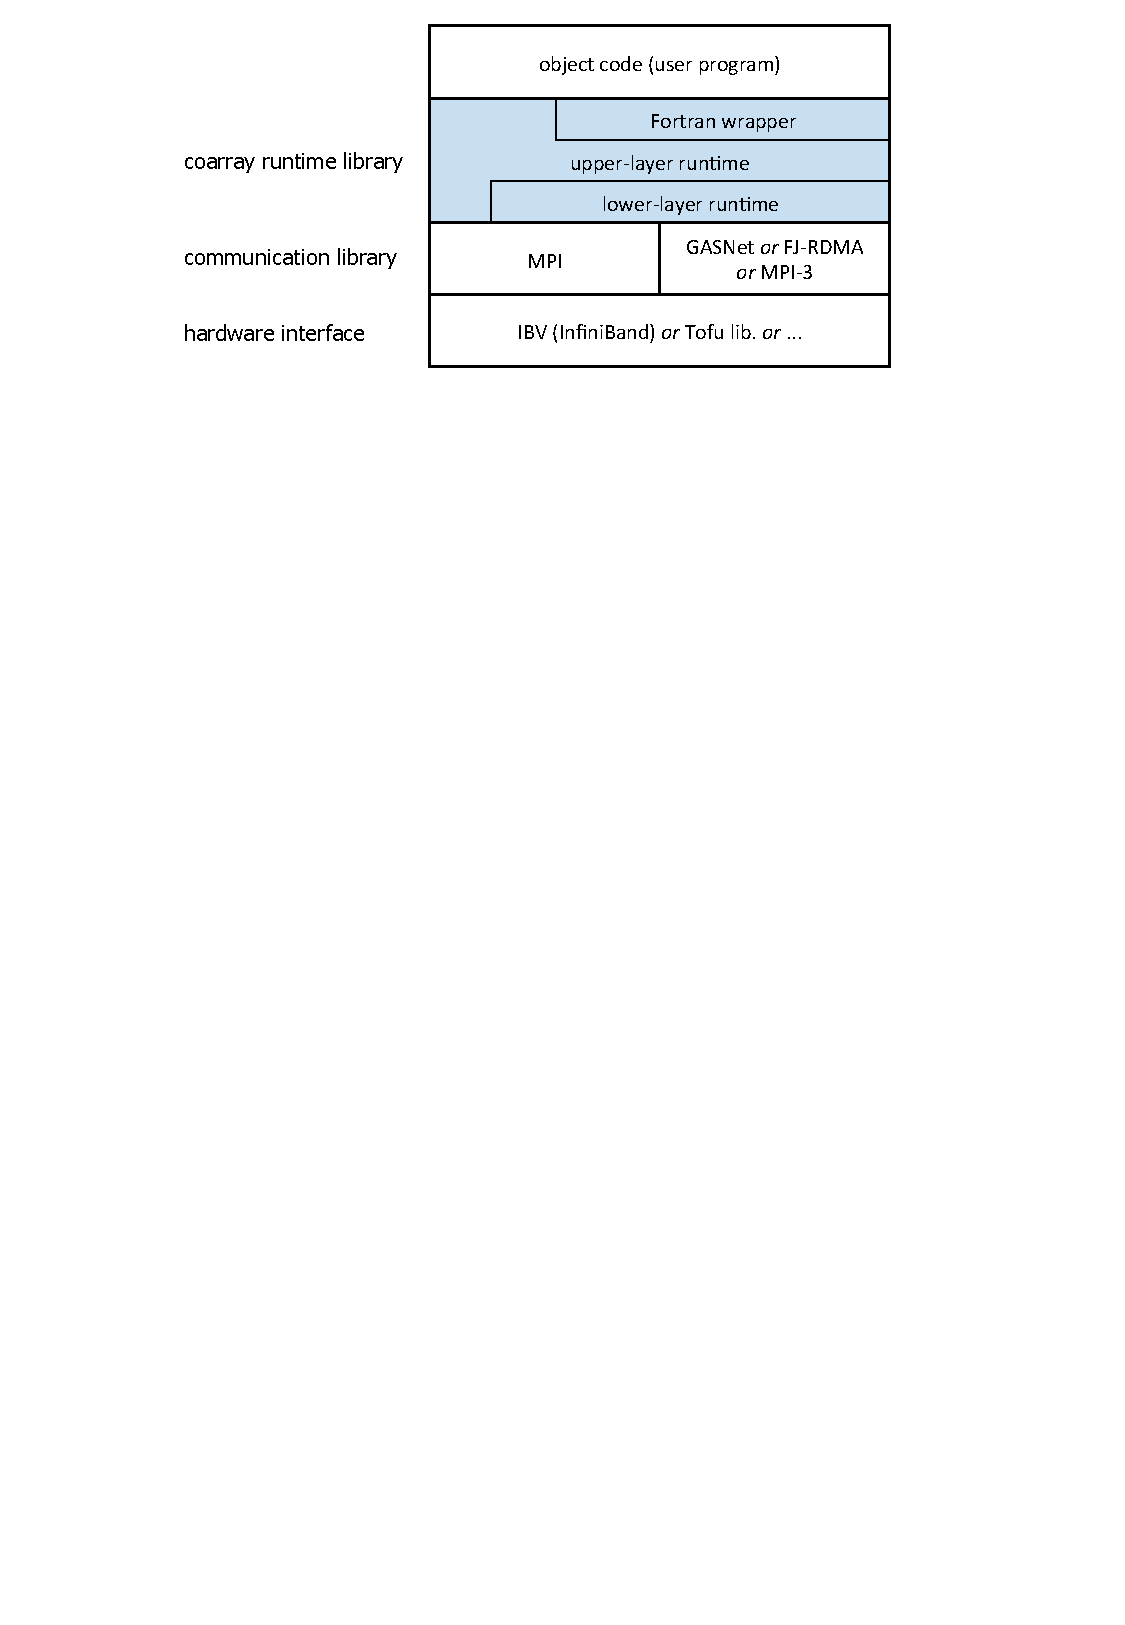
\includegraphics[trim=42mm 210mm 47mm 0mm, scale=0.7,clip]{figs/softstack-r2.pdf}}
    \mbox{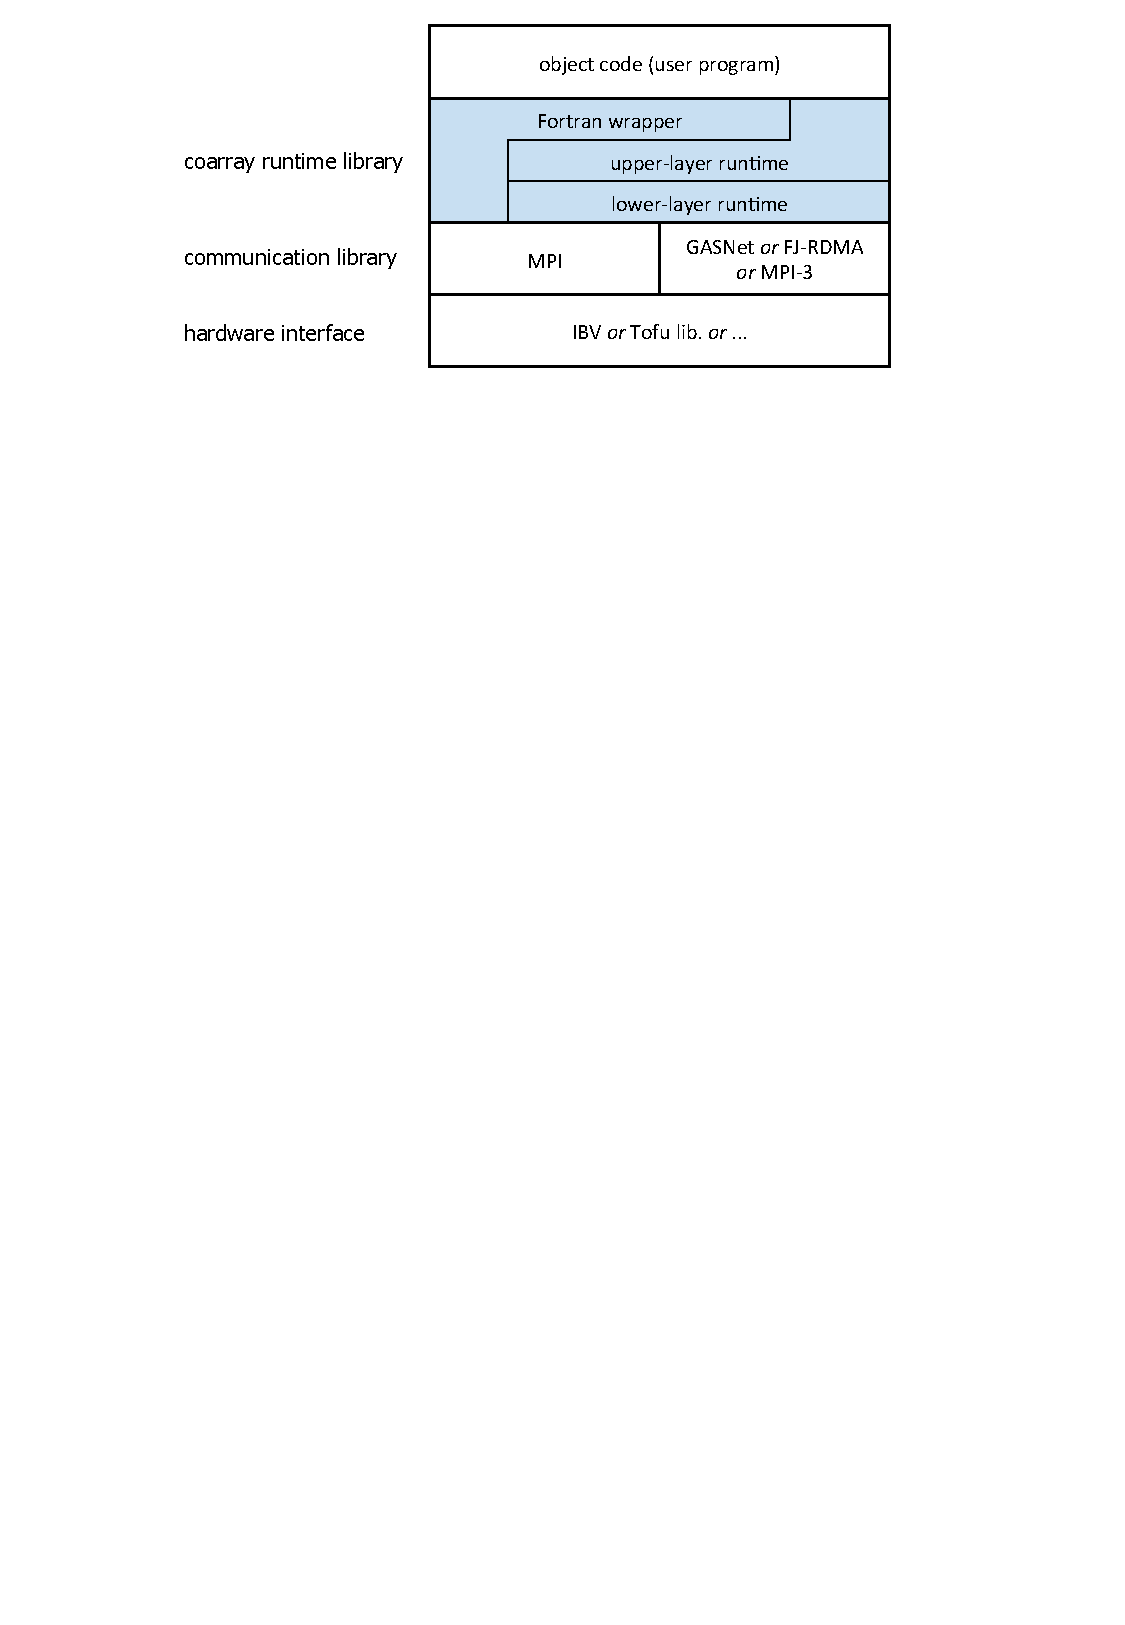
\includegraphics[trim=27mm 208mm 29mm 0mm, scale=0.7,clip]{figs/softstack-r4.pdf}}
    \caption{Software stack for coarray features}\label{fig:layer}
  \end{center}
\end{figure}


%===========================================================
\subsubsection{Fortran Wrapper}
%===========================================================

Each set of Fortran wrapper procedures has a generic name and dozens of corresponding specific names. For example, the object code contains a call to a function with
the generic name {\tt xmpf\_coarray\_get\_generic}.
If the data is a two-dimensional array of the 16-byte complex type,
the Fortran compiler selects the corresponding specific name 
{\tt xmpf\_coarray\_get2d\_z16} at compile time
and generates the object code by calling a ULR function 
by the specific name.

The Fortran wrapper accepts Fortran array notations as the arguments 
and the result variable and converts these notations into structures that can be handled in a runtime library written in C.
%
The Fortran wrapper also converts a C pointer to a Fortran pointer with the shape using
the Cray pointer.

The Fortran wrapper calls ULR procedures basically and 
calls MPI library functions directly for collective communications. 


%本実装では、Fortranの高級な仕様(配列記述や総称名手続き)を
%runtime libraryインタフェースとした。
%これにより、コンパイラが生成すべきオブジェクトインタフェースの数を
%数十分の一に削減してデータの型と形状をruntimeに伝えることができる
%ようになった。


%Actually, the interface is used through the Fortran~90 generic interface
%to ease the code generation by the coarray translator.
%For example, let us convert an {\tt ALLOCATE} statement
%{\tt allocate (a(1:10,2:19))}, where {\tt a} is an allocatable coarray of 16-byte,
%using object-ULR interface {\tt XMPCO\_malloc\_coarray}.
%The translator may generate a call to the generic procedure \\
%{\tt xmpf_coarray_malloc_generic(descriptor_of_a, a, 


%===========================================================
\subsubsection{Upper-layer Runtime (ULR) Library }
%===========================================================

The major role of ULR is performing the algorithms for coarray data
allocation/registration (\Sec{alloc}) and PUT/GET communications (\Sec{putget}).
Additionally, for atomic communications caused by intrinsic subroutines
{\tt ATOMIC\_DEFINE} and {\tt ATOMIC\_REF}, 
ULR calls the corresponding function of LLR after address calculation.

%===========================================================
\subsubsection{Lower-layer Runtime (LLR) Library}
%===========================================================

The LLR basically abstracts the difference between the communication libraries.
The only exception is the allocation and registration of coarray data.
Major functions are shown below.

\begin{itemize}
\item
Functions to allocate and register coarray variables,
and functions to register coarray variables that are already allocated.
They are alternatively used in the RS and RA methods and in the CA method.
Correspondingly, a set of functions to deregister and deallocate and
a set of functions to deregister are provided.

\item
Fundamental functions for RDMA-DMA GET communication and DMA-RDMA PUT communication.
It is assumed that both remote and local data are previously registered.
Blocking and non-blocking can be switched.
% and the only way to wait for
% the completion of the non-blocking communication is using the function
%corresponding to {\tt SYNC MEMORY}.

\item
Functions corresponding to image control statements, atomic subroutines,
and inquire functions.

\end{itemize}

The LLR also has the features for multi-dimensional data developed for the C 
implementation, which are not used in the Fortran implementation because
this implementation is solved in ULR.


%===========================================================
\subsubsection{Communication Libraries}
%===========================================================

MPI-3 can be selected for all platforms on which it is implemented. Coarrays are 
registered and deregistered at the start and end point of the MPI window. 
Coarrays perform one-sided communication by {\tt MPI\_Put} and {\tt MPI\_Get}
and are synchronized by {\tt MPI\_Win\_fence}. 
Implementation on MPI incurs certain costs for dynamic allocation of coarrays and 
waiting for communication completion.

GASNet can be selected for more advanced implementation over InfiniBand. 
Since allocation and registration of are inseparable and can be performed only once 
on GASNet, the implementation allocates and registers a pool of memory,
the size of which should be large enough to contain all static and allocatable coarrays.
The XMP runtime should allocate and deallocate coarrays without using the Fortran 
library but using the memory manager constructed for the pool.

FJ-RDMA can be selected for the implementation over the Tofu interconnection of 
the K computer and Fujitsu PRIMEHPC FX series supercomputers. 
Basically, each coarray is allocated by the Fortran library and 
the address is registered with the FJ-RDMA interface {\tt FJMPI\_Rdma\_reg\_mem}. 
The address is deregistered with {\tt FJMPI\_Rdma\_dereg\_mem} before being deallocated 
(freed) by the Fortran library. 
One-sided communication is performed with {\tt FJMPI\_Rdma\_put} and 
{\tt FJMPI\_Rdma\_get}.
%, which include confirmation of communication completion. <-- 本当? いつも?




